\chapter{Case Studies}

%do the usual introduction
% then explain wtf the idea is



\section{Scenario 1: Demand-Response Misinformation Campaign}
\label{demandresponsesection}
%First: Explain throuhout the scenario
%Then define assumptions
%Then define parameters
%Then simulation results
%This Scenario should also be the one with the total framework

With the increased usage of information and communication 
technologies (ICT), new methods of influencing
consumer demand patterns are possible. 
These can be used by electrical companies to change the 
demand curve over time, ideally to match energy consumption
with the energy created by renewable energis such 
as solar panels. 
This concept of changing the demand to match the 
available supply of electricity is called demand-response. 
One method to influence the consumer demand is by real time 
pricing (RTP). With RTP, the electricity prices change
dynamically based on the total electricity demand.
The price changes are then forwarded to the customers with ICTs, 
who are thus informed of the price changes.
The idea of RTP is that consumers change their electricity demand
by shifting activities with a high electricity usage, 
such as washing clothes or cooking, to time periods 
where the total electricity supply is higher and thus the prices
are lower. This leads to reduced peak energy consumption. 
RTP was already used in a variety of programs
under real life conditions \cite{barbose2004survey}.
Studies showed the benefits of such programs \cite{albadi2008summary}.

Problematic is if a false pricing rumor spreads through social media.
In 2022, changes in the verification policies of Twitter lead to users being able 
to impersonate well-known brands such as Pepsi, leading to Twitter 
users being unable to determine which social media channels were
posting trustworthy information \cite{twitterchaos}. One user could
have used the policy changes of Twitter to impersonate 	utility companies
and to advertise a false reduction of energy prices, leading to customers
believing the information and increasing their energy consumption as a 
reaction. Another possibility would be that hackers would force access to the
social media profiles of utility companies and start sending false 
information to its customers. Hackers were already able to gain access
to the social media profiles of multinational companies in the past
\cite{twitterhacker}. Hackers could also spread misinformation in regards
to a false reduction in prices, thus leading to changing consumer demand.

Based on the information, a possible scenario could be that hackers would
access the social media profiles of a well-known utility company
to spread the information that the energy prices would be reduced by 
a signifiant factor at a specific time. An example tweet is shown in 
Figure \ref{demandtweet}. This information would then be 
spread around social media, reaching many customers of the company.

\begin{figure}[!ht]
    \center
    
\includegraphics[scale=.4]{figs/eondemandresponse.png}
    \caption{Example tweet posted by hackers pretending to be an utility company}
    \label{demandtweet}
\end{figure}

Given the description of the scenario, multiple assumptions can be made.
First, we can assume that the time where an entity receives the information
about the price reduction does not correlate with the time it will act on
it. Furthermore, since it is a widespread information propagation scenario,
we can use a similar information propagation event to analyze the 
results of the total framework. Thus, the information propagation
parameters do not need to be defined. Furthermore, one work estimates 
the price elasticity of electricity in Germany to be $-0.4310$
\cite{priceelasticity}. 
This means that a price reduction of $1\%$
on the electricity price would could lead to a $0.43\%$ increase in
electricity consumption. From this, we can assume that consumers 
respond well to such price reduction programs. Thus, we can also assume 
that many people will act on the information.

To estimate the information propagation parameters with the framework,
example social media data is necessary. However, there are no real examples
for social media information spread events which affected the power demand.
Thus, other information spreading events are used to estimate 
realistic propagation parameters. The dataset used for this scenario
was the Typhoon Haiyan dataset \cite{david2016tweeting}. In this
dataset, $2.753.230$ twitter posts and their published dates were collected
to analyze communication during a disaster. The twitter posts were collected
between November 8, 2013 and November 26, 2013. This means that the 
information propagation for this dataset progressed over multiple days.
The propagation curve and the estimated infection curves can be seen in 
Figure \ref{propagationestimationtyphoon}. In the figure, it can be seen 
that the parameter estimation algorithm models the infection progress
well, ignoring outliers such as the maximum value of the true information
propagation progress. Furthermore, the
information is assumed by the framework to have a high credibility 
of $\alpha=1$. The transmission rate is estimated to be average with 
$\beta=0.65$.
Since the infection process is slow and progresses over 
multiple days, the verification parameter is
low with $p_{\mathrm{verify}}=0.001$. Last, the degree-to-node ratio
is also low with $\frac{k'}{N'}=0.006$.


\begin{figure}[!ht]
    \center
    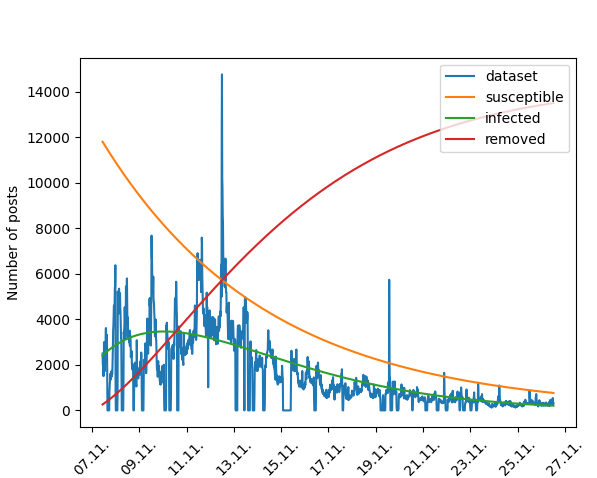
\includegraphics[scale=.95]{figs/parameter_estimation.png}
    \caption{Information propagation progress for the Typhoon dataset 
    and estimated infection process}
    \label{propagationestimationtyphoon}
\end{figure}

Besides the propagation parameters, which are estimated by the framework,
the system parameters $p_{\mathrm{will\_act}}$ and 
$p_{\mathrm{power\_usage}}$ need to be defined. Since the information 
propagated in the scenario
is believeable and we assume that customers respond well to price 
reduction programs, we can also assume that the two probabilities are 
reasonably high. For this simulation, values of $p_{\mathrm{will\_act}}=0.8$ and 
$p_{\mathrm{power\_usage}}=0.8$ were chosen. Furthermore, this scenario
is given for only one utility company and not for the whole 
energy market. We assume that $50\%$ of the households of a city belong
to an utility company X. Last, since the scenario would both be 
well-received by the entities and it is a believeable scenario, 
entities may also share the information with its neighbors even if
cannot act on the information. A reason for why an entity cannot act 
on the information is that it is the customer of another utility company.
This scenario considers the household appliances which are energy-intensive.
The config file of the scenario with all appliances considered in this
scenario can be found in the Appendix in Listing \ref{scenario1config}.

% next ideas: average over multiple seeds
% check out how unstable the simulation is
% then find out how the simulation acts based on the other two probabilities

To evaluate this scenario, the simulation was run five times with five 
different seeds used for the random probability calculations to ensure
different results. In addition, the simulation generates a social media
graph model with $1000$ nodes. The results of the simulation 
can be seen in Figure \ref{firstscenariobasicresult}.
The left plot shows the power consumption of the model. The right 
plot shows the infection progress during the simulation.
The lines in both plots show the average values over all simulations and 
the lighter-colored areas around the lines show the minimum and maximum values
over all simulations. 


\begin{figure}[!ht]
    \center
    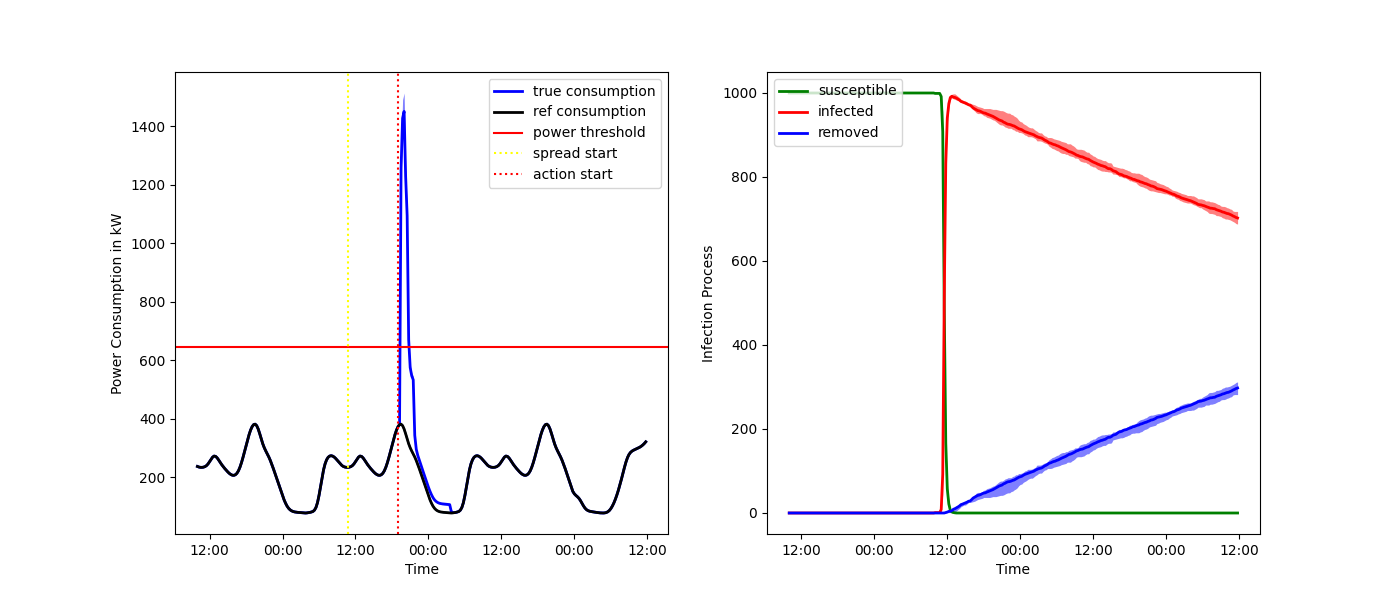
\includegraphics[scale=.53]{figs/eval/scenario1/basic_run.png}
    \caption{Simulation results for the first scenario}
    \label{firstscenariobasicresult}
\end{figure}

For the power consumption curve in Figure \ref{firstscenariobasicresult}, 
it is noticeable
that the power consumption spike generated by the infection is directly
after the time where entities can reasonably start acting on the information.
In addition, few hours after the spike, the excess power consumption
reduces to an amount that the infractructure can handle. 
The reason is that even though there are still many infected entities
in the system, the duration in which specific household appliances
such as dishwashers run are limited. Thus, after running the specific
appliances, they do not consume any more power. The result of the simulation
can be compared to the results of the simulation shown in 
Figure \ref{firstscenariobasicevchange}, where the duration of the 
appliance \code{electric\_car} is changed from \code{32} to \code{1000}.
Figure \ref{firstscenariobasicevchange}, it is noticeable 
that there is a constant overconsumption compared to the reference
power consumption shown with the black line since the \code{electric\_car}
appliance does not finish using power.
Furthermore, the 
results of the framework are robust and show little variance over the
different simulations. 
Infection curve in the right plot shows a rapid increase in infected 
individuals, followed by a slow, linear decrease in infected entities.
The rapid increase cannot be explained by the 
infection curve shown in Figure \ref{propagationestimationtyphoon}.
The Figure can only explain the slower decrease, since the infection
curve shows a slow decrease over a week. This mismatch between
the system-wide infection curve in Figure \ref{propagationestimationtyphoon}
and the infection curve generated by the graph-based algorithm 
in Figure \ref{firstscenariobasicresult} can have two reasons. 
First, the initialization assumptions of the simulation may be false.
In Section \ref{rulebasedpowerconsumption}, the simulation model
is defined with one node belongin to the \textit{Infected} class.
However, in Figure \ref{propagationestimationtyphoon}, it
is visible that the number of infected individuals at the 
time $t=0$ is more than one. This may lead to mismatches 
in the results. Second, the assumptions given in Section 
\ref{parameterestimationalgo} could be false. For example, 
the graph model is simplified such that all nodes are considered
to have the degree $k$. However, since the generated graph models 
are clustered, there are nodes that have the degree $k'\gg k$. 
If these are infected, they are able to infect more nodes compared
to other nodes that are less connected. Thus, the infection 
proceeds quicker than expected.

\begin{figure}[!ht]
    \center
    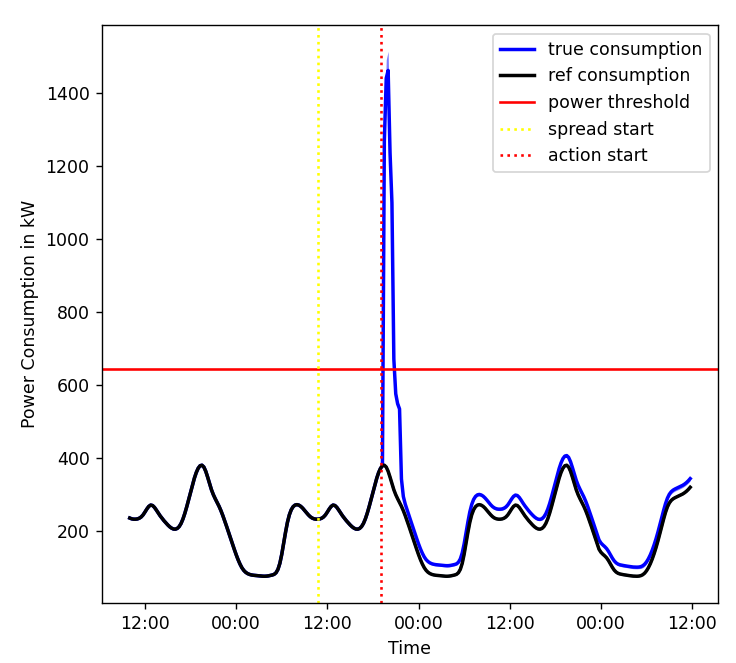
\includegraphics[scale=.5]{figs/eval/scenario1/longev.png}
    \caption{Simulation results when increasing the duration to 
    charge electric cars to 1000}
    \label{firstscenariobasicevchange}
\end{figure}

Next, the sensitivity of the propagation process 
in regards to the variable $\alpha, \beta, p_{verify}$ 
was analyzed. For the evaluation, one parameter was changed
while the other two parameters were fixed.
The fixed values for the parameters were 
$\alpha=0.4, \beta=0.2, p_{verify}=0.2$. 
The infection progress, the immunization progress 
and the maximum power usage were analyzed.
The simulation was run five times for each parameter
value to ensure different simulation results. The 
averages of the simulation results are shown in the 
Figures \ref{scen1variablealpha},
\ref{scen1variablebeta} and \ref{scen1variablepverify}.


\begin{figure}[!ht]
    \centering
    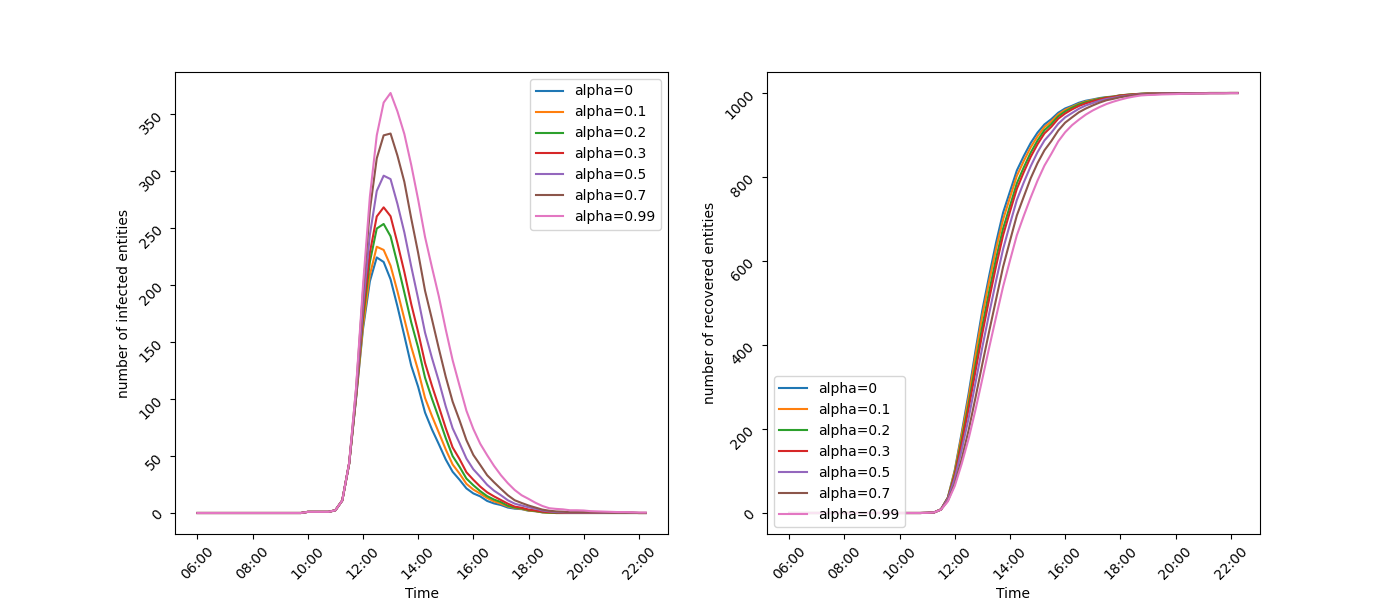
\includegraphics[scale=.5]{figs/eval/scenario1/alpha_mix.png}
    \caption{Infection process with changing variable $\alpha$}
    \label{scen1variablealpha} 
\end{figure}

\begin{figure}[!ht]
    \centering
    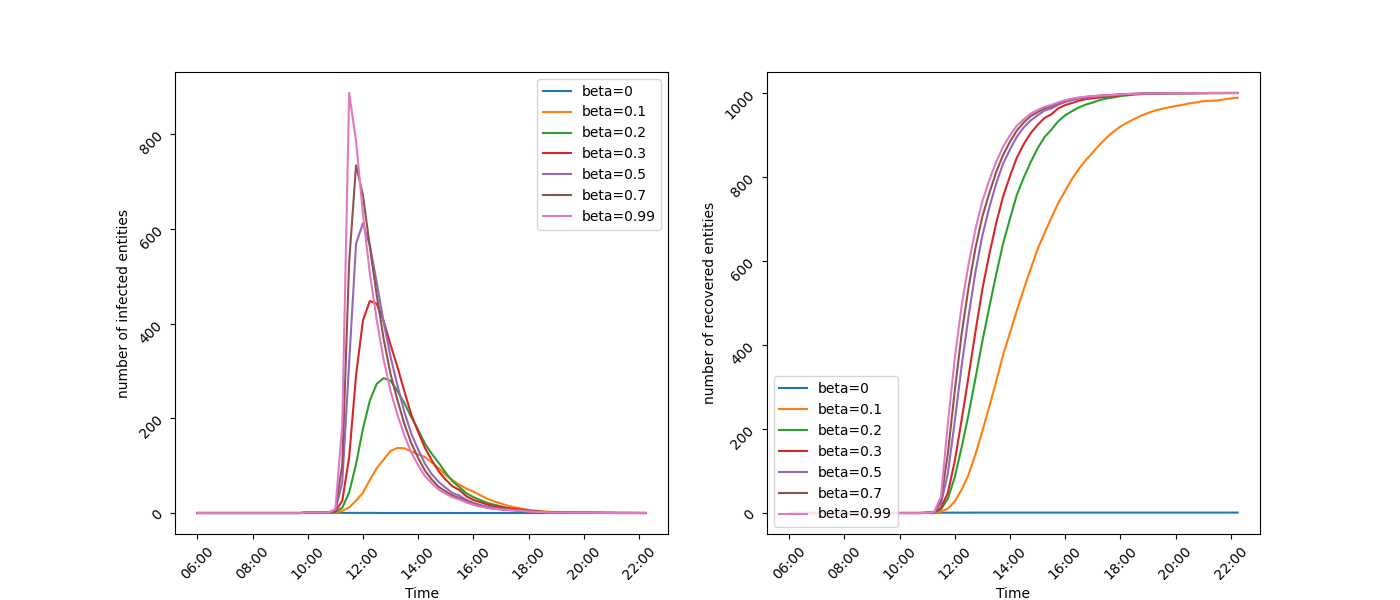
\includegraphics[scale=.5]{figs/eval/scenario1/beta_mix.png}
    \caption{Infection process with changing variable $\beta$}
    \label{scen1variablebeta} 
\end{figure}

\begin{figure}[!ht]
    \centering
    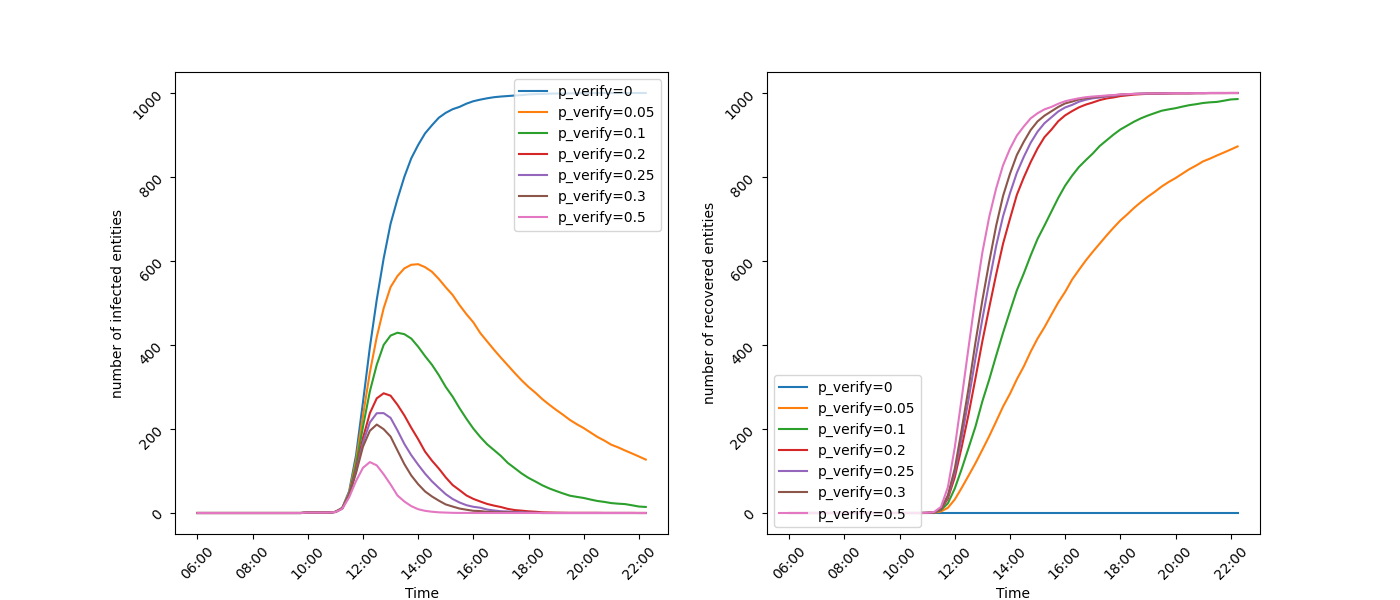
\includegraphics[scale=.5]{figs/eval/scenario1/verify_mix.png}
    \caption{Infection process with changing variable $p_{verify}$}
    \label{scen1variablepverify} 
\end{figure}


In Figure \ref{scen1variablebeta}, the infection process with
variable $\alpha$ are shown. It is observable that with the given
parameters $\beta, p_{verify}$, the infections process is
not very sensitive to changes in $\alpha$. The number of infected
entities tend to reduce with lower $\alpha$, but the changes
are low compared to the other propagation parameters.
In Figure \ref{scen1variablebeta}, it is evident that the
infection process is more sensitive to changes in 
$\beta$ compared to $\alpha$. The maximum number of infected 
individuals increases with higher values for $\beta$.
The number of recovered individuals also increases with higher
$\beta$, suggesting that the system is more dynamic with higher 
$\beta$, increasing the speed that susceptible entities
become infected and later recover. Moreover,
the infection process rises and falls in a greater rate with 
higher $\beta$. In Figure \ref{scen1variablepverify},
it can be observed that the propagation process is also 
sensitive to changes in $p_{verify}$. The number of infected 
individuals reduce with higher $p_{verify}$, since a higher
number of entities can get informed with the true information
with a higher $p_{verify}$ and can change their state to 
\textit{Removed}. As a consequence, the number of removed
entities increases faster with higher $p_{verify}$.
In general, it is visible that the the number of infected
individuals increases quickly, independently of any
changes in variables. The reason lies in the method to 
calculate the probability of the states of the entities.
At the beginning of the simulation, there are no recovered
entities, only susceptible and infected individuals.
Thus, considering the equations shown in Equation 
\ref{modified-SIS-table-equations}, we can assume
for the initial stages of the propagation process
that for a significant amount of nodes the 
parameters $f_i, g_i$ have the values 
$f_i=\beta, g_i=0$. Consequently, most nodes immediately 
change their state from \textit{Susceptible} 
to \textit{Infected} for a high value of $\beta$.
This means that the maximum number of infected 
individuals is reached in the early stages of the 
infection progress, followed by a slower decrease
in infected individuals. 


Another set of parameters of interest for the evaluation
are the parameters which delay or prevent excessive
power usage. These are the parameters $p_{\mathrm{power\_usage}},
p_{\mathrm{will\_act}}, p_{\mathrm{available}}$.
The sensitivity of the simulation results to these parameters
was tested by changing one of the parameters, leaving 
the other parameters fixed with the probabilities
$p_{\mathrm{power\_usage}}=1,
p_{\mathrm{will\_act}}=1, p_{\mathrm{available}}=1$.
The simulation was run five times with different seeds 
to ensure different simulation results. The 
averages of the simulation results are shown in 
Figure \ref{scen1variablepowervals}.
The simulated power usage values were substracted with the 
reference power 
usage values, only showing the excessive power usage
in the Figure.

\begin{figure}[!ht]
    \centering
    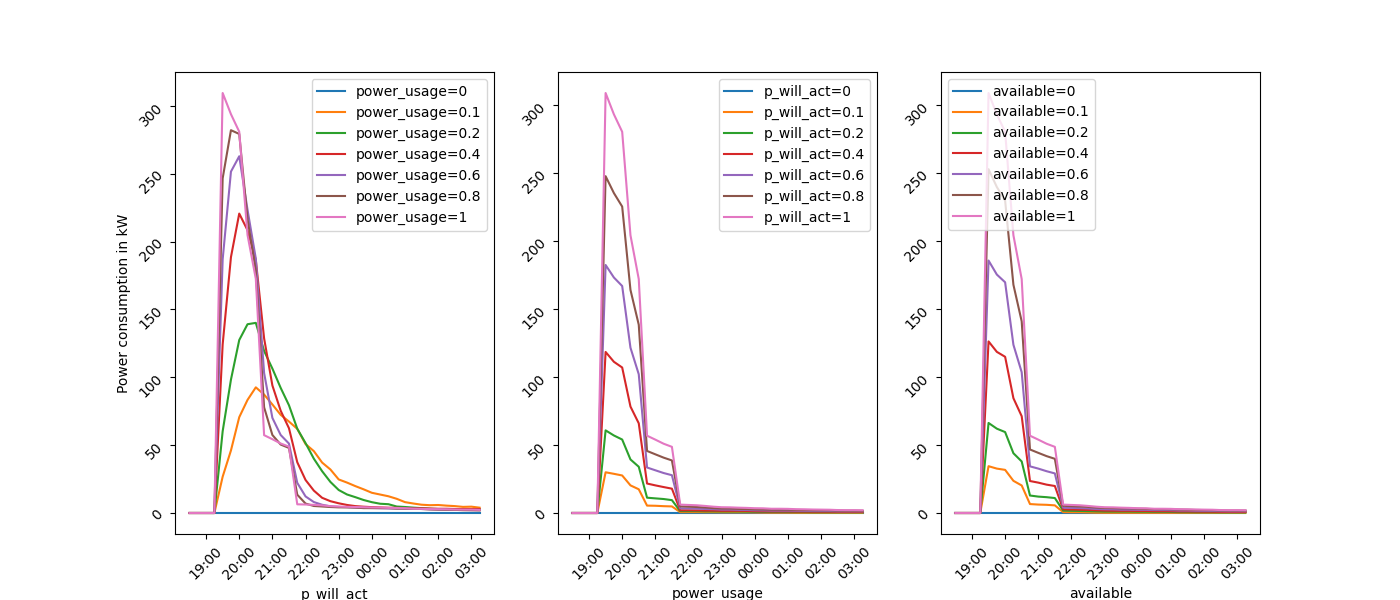
\includegraphics[scale=.5]{figs/eval/scenario1/powervars.png}
    \caption{Excess power usage curve with different 
    $p_{\mathrm{power\_usage}}, p_{\mathrm{will\_act}}, 
    p_{\mathrm{available}}$}
    \label{scen1variablepowervals} 
\end{figure}

In Figure \ref{scen1variablepowervals}, it can be observed that
the the excess power usage is very sensitive to changes in all
three parameters. If any of the parameters is $0$, then no
excess power consumption occurs. The reason is that 
for an entity to consume more power, it needs to fullfill
all conditions which are related to the three 
probabilities. If one of the probabilities is $0$, then 
no entity can fulfill the condition related to the 
specific probability. Moreover, with increasing parameter
values, the excess power consumption increases. The 
cause is that with higher probability values, it is 
easier for the entities to fulfill the condition
related to the specific probability. As a 
consequence, more entities are able to consume more 
power and the total excess power demand increases.
In addition, it can be seen that the excess power 
demand curve is wider for the parameter 
$p_{\mathrm{power\_usage}}$ than for the other parameters.
The reason is that the parameter delays the 
excess power consumption, it does not prevent it.
This means that with reasonably low values for 
this parameter, the excess consumption curve 
has a lower peak, but also a wider slope.
Therefore, a low value for $p_{\mathrm{power\_usage}}$
stretches the power consumption curve, leading
to a less critical, but longer lasting 
overconsumption period. This can also be seen in Figure 
\ref{scen1variablepowerusage}, where lower 
$p_{\mathrm{power\_usage}}$ leads to 
a longer, but less high overconsumption period.
Therefore, it can be assumed that synchronized 
behavior can lead to power demand issues.
Synchronized behavior can be described 
as the phenomenom where different individuals
consciously or unconsciously
perform the same actions at the same time.
This problem is already known and was
already the topic of other research works
\cite{lei2014impact} \cite{walker2014dynamics}
\cite{gebhard2022monitoring}.

\begin{figure}[!ht]
    \centering
    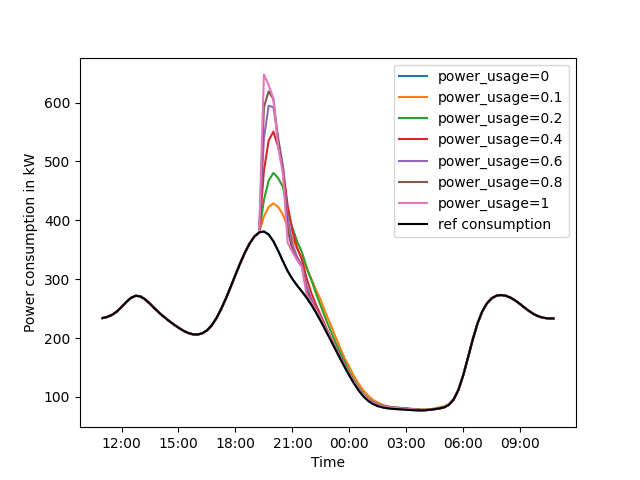
\includegraphics[scale=.6]{figs/eval/scenario1/powerusage.png}
    \caption{Excess power usage curve with different values for 
    $p_{\mathrm{power\_usage}}$}
    \label{scen1variablepowerusage} 
\end{figure}

\section{Scenario 2: Coordinated Action of Extremists 
against the Electrical Grid}

Echo chambers on various social media websites allow people to 
hear biased opinions and news which confirm their views on 
various topics \cite{terren2021echo}. This leads to political
polarization and extremism \cite{van2022banality}.
These people in turn can try to fight the established political
system. Research shows that social media influence people
to commit hate crimes \cite{muller2021fanning}.
In general, the number of violent incidents caused by
extremists, specially right-wing extremists, is rising 
\cite{koehler2016right}. 
Most of the criminal acts caused by political extremism 
in germany are in the fields of property damage, 
propaganda crimes, insults and hate speech \cite{bmicrimestatistics}.
But extremists also cause more serious crimes. In 2022,
right-wing extremists planned to sabotage the electrical grid 
infrastructure by destroying power lines \cite{anschlagstrom}.
Thus, it can be seen that critical infrastructure may also be a target
for political extremists. 

Another way to target critical infrastructure is with a coordinated
actions which in its sum can damage the infrastructure. The 
reasons for a group of people to take such action may be harmless,
such as the Earth day, where people where encouraged to switch off their 
lights and appliances to save energy \cite{earthday}.
But extremists could also synchronize their actions to reduce their
power consumption to a minimum, thus mismatching electricity supply
and demand by a considerable degree. Electricity companies would 
then need to deal with a sudden surplus of electricity.

Given the previous information, a possible scenario could be 
that extremists plan to turn off all their electrical devices at 
a specific time to destabilize the electrical infrastructure. The
time would be announced in advance. An example message spread by
these extremists can be seen in Figure \ref{schwurbler}.

\begin{figure}[!ht]
    \center
    
\includegraphics[scale=.7]{figs/schwurblerchat.png}
    \caption{Example message posted by extremists on Telegram}
    \label{schwurbler}
\end{figure}

Given the description of the example scenario, multiple assumptions can be drawn.
First, this scenario also assumes that the time where an entity receives the
information does not equal to the time where it acts on the information.
Furthermore, this scenario is unlikely to make large parts of the population
act on the information since it is assumed that only a small minority
of the population will act on extremist information. But the small 
minority which is open for such ideas are likely to act on the 
messages that they receive.
This means that the parameter $p_{\mathrm{available}}$ has a low value,
whereas $p_{\mathrm{power\_usage}}, p_{\mathrm{will\_act}}$
have high values. For this scenario, the values 
$p_{\mathrm{available}}=0.2, 
p_{\mathrm{power\_usage}}=1, p_{\mathrm{will\_act}}=1$
were chosen.
Moreover, it is expected that infected individuals will not 
believe in any information that goes against the original message.
Therefore, it is assumed that $p_{\mathrm{verify}}=0$. Next, it
can be considered that the information is believable to 
the affected population and that it is quickly spread by 
the infected entities. Thus, it is assumed that $\alpha=1, \beta=1$.
However, the information is not believeable to the people 
who are not open to extremist messages. Thus, the 
parameter \code{fringe} is set to \code{true}.
Next, it is assumed that all infected entities 
stop consuming power and their demand decreases to zero. Thus,
the power usage factor \code{factor} is set to zero.

To analyze the scenario, the simulation was run five times with five 
different seeds. Furthermore, a model with $1000$ nodes was used 
for the evaluation. The results of the simulation can be seen in
Figure \ref{schwurblerresults}. In the Figure, it can be 
observed that the amount of infected individuals is not high.
From $1000$ nodes, only $200$ get infected. The reason is 
that $p_{\mathrm{available}}=0.2$, thus only $20\%$ of the nodes
can get infected. In addition, it is visible that the results 
are not very robust. The results change heavily in different 
simulations. The reason is that depending on the network structure
and which nodes can get infected and will act on the information, 
the infected nodes may not be able to infect all other nodes
that could get infected. Nodes that can get infected may be 
connected by nodes that are not susceptible to the conspiracy 
theory, which does also not forward the message to other nodes
open to the conspiracy theory, thus limiting the 
spread of misinformation.
Moreover, it can be seen that the amount of underconsumption
is higher in peak load periods compared to periods with 
lower load. This makes sense since infected households would 
normally use more energy during peak load times. Their absence
means that a higher amount of power load demand is missing 
during these periods. Additionally, the decrease in demand 
changes immediately after the moment where the entities 
should change their action. This means that the changes 
in power demand are abrupt and could surprise the responsible 
power suppliers.

\begin{figure}[!ht]
    \center
    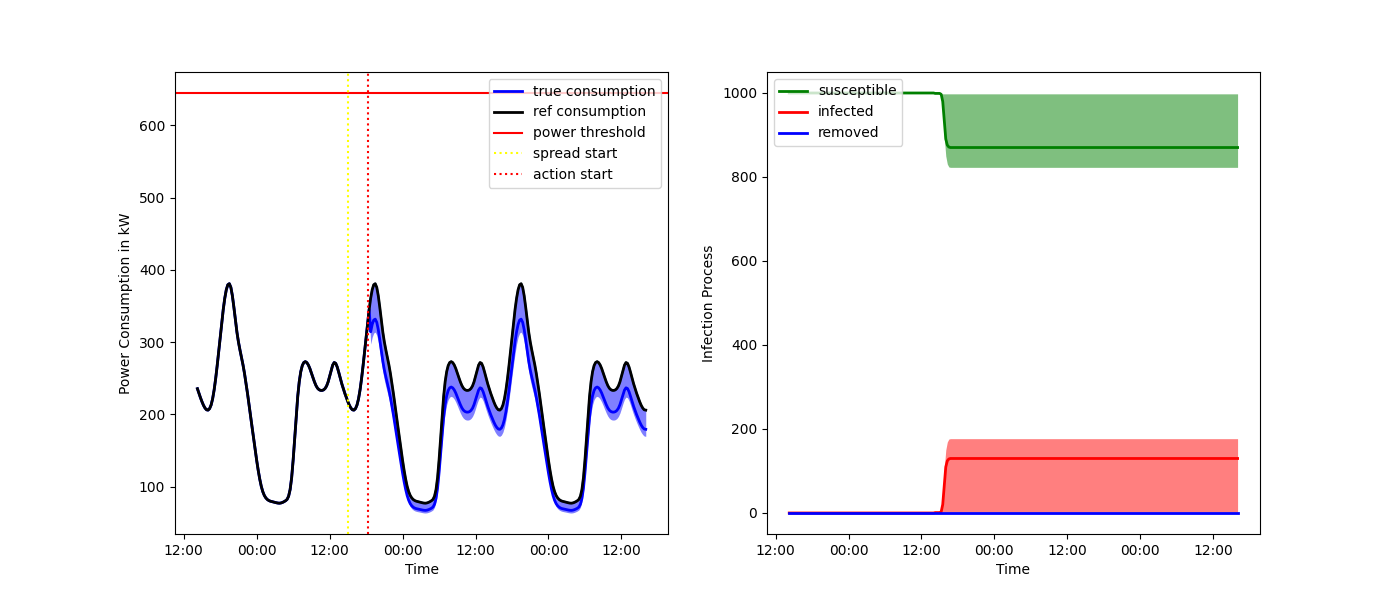
\includegraphics[scale=.55]{figs/eval/scenario2/basicplot.png}
    \caption{Simulation results for the second scenario}
    \label{schwurblerresults}
\end{figure}

In Figure \ref{schwurblerresults}, it could be seen that 
the results of the simulation are not robust. To analyze the 
robustness of the simulation in regards to the parameter
\code{fringe}, a second simulation was run where the 
\code{fringe} parameter was set to \code{false}. 
The simulation was run five times with five different seeds
to ensure different results. The simulation results can be
seen in Figure \ref{schwurblerresults2}. It
can be observed that if \code{fringe} is \code{true}, then 
the simulation results get less robust. The reason is 
that the infection process may be hindered and thus not
all nodes can get infected. The \code{fringe} parameter was 
implemented by making nodes which are not available and thus
do not use additional power consumption
also not able to forward the information to other nodes.
Thus, these nodes can hinder the information propagation process.
However, this idea may not be realistic. Smaller communities,
such as extremist communities, may 
be tightly connected. Therefore, there may be no information 
barriers that could hinder the flow of information between 
entities that are open for this kind of information.



\begin{figure}[!ht]
    \center
    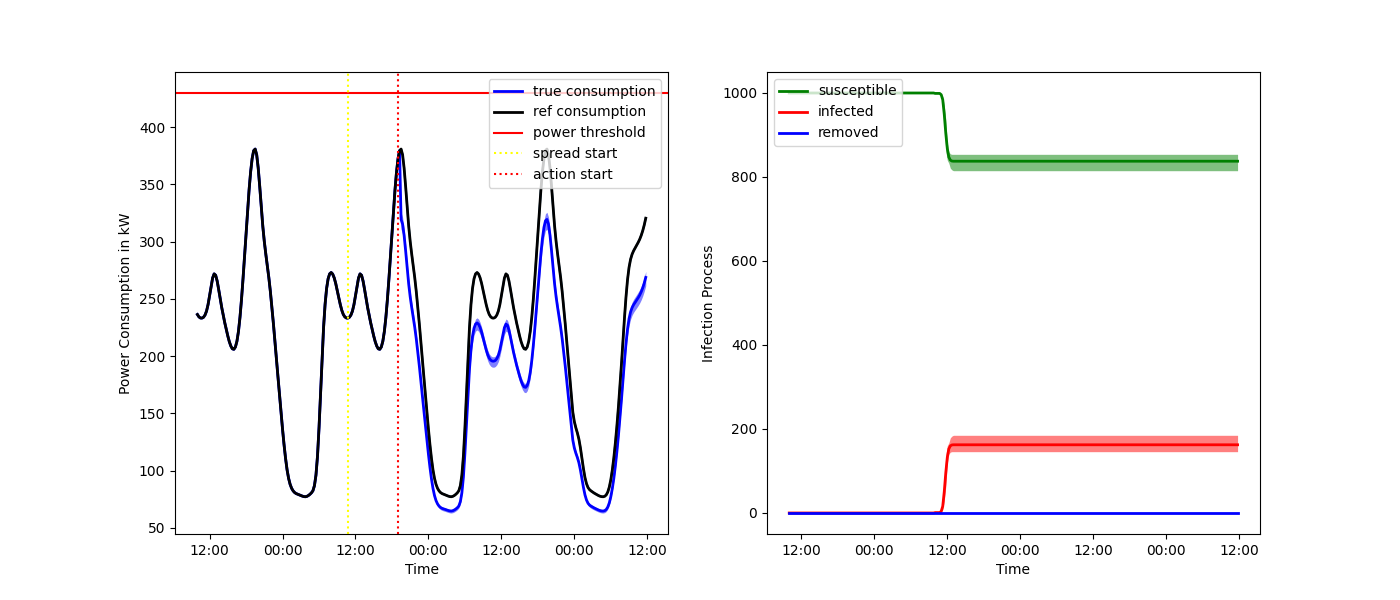
\includegraphics[scale=.55]{figs/eval/scenario2/fringeoff.png}
    \caption{Simulation results when all nodes forward the information}
    \label{schwurblerresults2}
\end{figure}


\section{Scenario 3: Mass Evacuation of a City due to a Disaster}

Sometimes the conditions under a disaster get so extreme that 
authorities choose to order the evacuation of the affected population.
For these types of evacuation, the autorities may use emergency channels 
to inform the population of the evacuation.
But people may also choose to leave the city in masses on their own accord.
The information of a possible disaster, such as a wildfire, reaching the
city soon or other disasters such as a widespread terrorist attacks 
in the city.
If people decide to leave their homes to flee from the disaster, they 
will mostly use their cars as the mode of transportation.
In the future, the increased adoption of electric vehicles (EV)
may lead to people needing to recharge their EVs if they wish 
to drive them. An evacuation could lead to many people charging
their cars at the same time, thus creating excess demand that 
the infrastructure is unable to handle. 

Given the previous assumptions, a possible scenario could be that 
rumors about a wildfire spreading towards a city leads to people
trying to leave the city in masses. In addition, a significant 
amount of people drive EVs, thus giving them the need to charge
their cars before they are able to leave the city. An example
tweet spreading the rumor can be seen in Figure \ref{firetweet}.


\begin{figure}[!ht]
    \center
    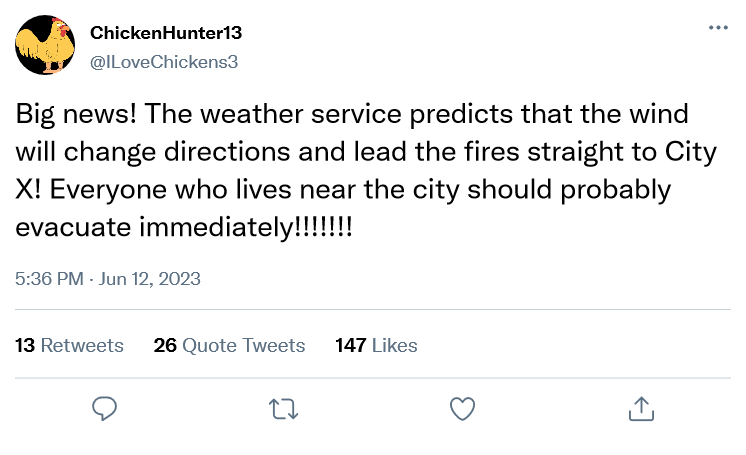
\includegraphics[scale=.4]{figs/firenews.png}
    \caption{Example tweet posted by an anonymus user on Twitter}
    \label{firetweet}
\end{figure}

Given the example scenario, multiple assumptions for the simulation can
be made. First, it can be assumed that the time where an entity receives
the information equals the time where the entity will act on it.
Next, It can be assumed that the information will be shared very quickly.
Furthermore, it is assumed that most people will act on the information,
since they will fear for their lives.


\section{Scenario 4: Mass Showering after a Chemical Accident}
%This Scenario should also be the one with the total framework

With the increasing usage of ICTs in the population, it allows for 
new methods to communicate with people about extreme circumstances
such as natural disasters or other catastrophes. In 2022,
a new warning system called Cell Broadcast was introduced in Germany
\cite{techrichtlinie}. Cell Broadcast can be used to warn the population
of emergencies by sending all cellphone users in the 
region of interest a message with a loud alert tone.
Furthermore, with the growing threat of climate change, many countries
are adopting measures to reduce the societal impact on the
climate. One of the fields that these measures affect 
are heating technologies. Currently, $75\%$ of the households 
heat with fossil fuels \cite{bdewhouhseholds}. 
However, there are measures being 
implemented to increase the usage of renewable resources such 
as electricity from solar panels in residential heating
\cite{heizungsgesetz}. Therefore, the number of households 
using electricity for heating are increasing, with 
$57\%$ of newly build houses installing 
heat pumps, which use electricity to heat
\cite{heatingpumps}.

Germany has one of the biggest chemical industry sectors in the world.
It is home to big chemical factories in cities such as Ludwigshafen and
Darmstadt. Areas with chemical factories have the risk of being
affected by chemical accidents.

A possible scenario would be that a chemical accident in a 
factory near a major city would lead to dangerous chemicals 
leaking out. These chemicals would spread through the air 
and adhere to the skin of humans, leading to serious 
health problems if they stayed on the skin for too long.
Thus, the city's government would use Cell Broadcast to
instruct the population to close their windows and 
to take a shower to remove the chemicals from their bodies.
Therefore, most people would take showers at the same time,
using electric heat pumps to heat up their water to shower.
An example message can be seen in Figure \ref{warningmessage}.

\begin{figure}[!ht]
    \center
    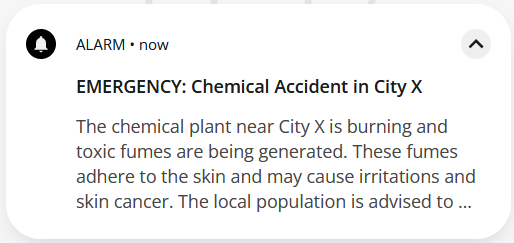
\includegraphics[scale=.7]{figs/emergencychemical.png}
    \caption{Example warning message received via Cell Broadcast}
    \label{warningmessage}
\end{figure}

Given the scenario description, multiple assumptions can be
made for the simulation.
First, it is assumed that since Cell Broadcast is used, the simulation
will reach all entities in the city at the same time.
Furthermore, since the information comes from a verified channel,
all entities will act on the information. Also, the time where the
entities receive the information is also the time where they will act
on it.
Moreover, since this scenario is a synchronous event, we can define that the
maximum number of infected individuals at the same time equals
the total number of entities in the system, thus $I(t_{max})=N$.
Consequently, the usage of the simulation work is not necessary
and the results of this scenario can be calculated manually.
Darmstadt is chosen as the example city for this scenario analysis.

Darmstadt is a city with $89.194$ households by 2020 
\cite{statistadarmstadt}. The 
Federal Association of the Energy and Water Industry
(Bundesverband der Energie- und Wasserwirtschaft (BDEW)) 
says that $3\%$ of the households in Germany currently use
heat pumps for heating. Therefore, we can assume that 
$0.03 \cdot 89.194 \approx 2675$ households currently use 
heat pumps. An average heat pump uses ca. $2$ kWh per hour, 
or $0.5$ kWh per $15$ minutes.

If we assume that all households in Darmstadt receive 
a message at the same time via Cell Broadcast and that
every household takes a hot shower for 15 minutes,
we can calculate that there will be an additional 
demand of $0.5kWh \cdot 2675 = 1337.5 kWh $ for these 
15 minutes. If an average household uses $3900 kWh$ 
per year and $0.44kWh$ per hour, then using the heat pump 
would double their power consumption for a short time.

